%!TEX root = ../luanvan.tex
\chapter{Xây dựng hệ thống}

\section{Mô tả bài toán}

Bài toán đặt ra nhu cầu quản lý thông tin của người cấp, người được cấp VBCC để số hóa các quy trình cấp VBCC, sở hữu VBCC, chia sẻ thông tin xác thực VBCC có liên quan đến thông tin cá nhân của người được cấp VBCC theo các quy định hiện hành về bảo vệ bí mật thông tin trong môi trường trực tuyến.
Sơ đồ bài toán được minh họa như hình \ref{fig:vbcc}.

\begin{figure}[htbp]
\centering
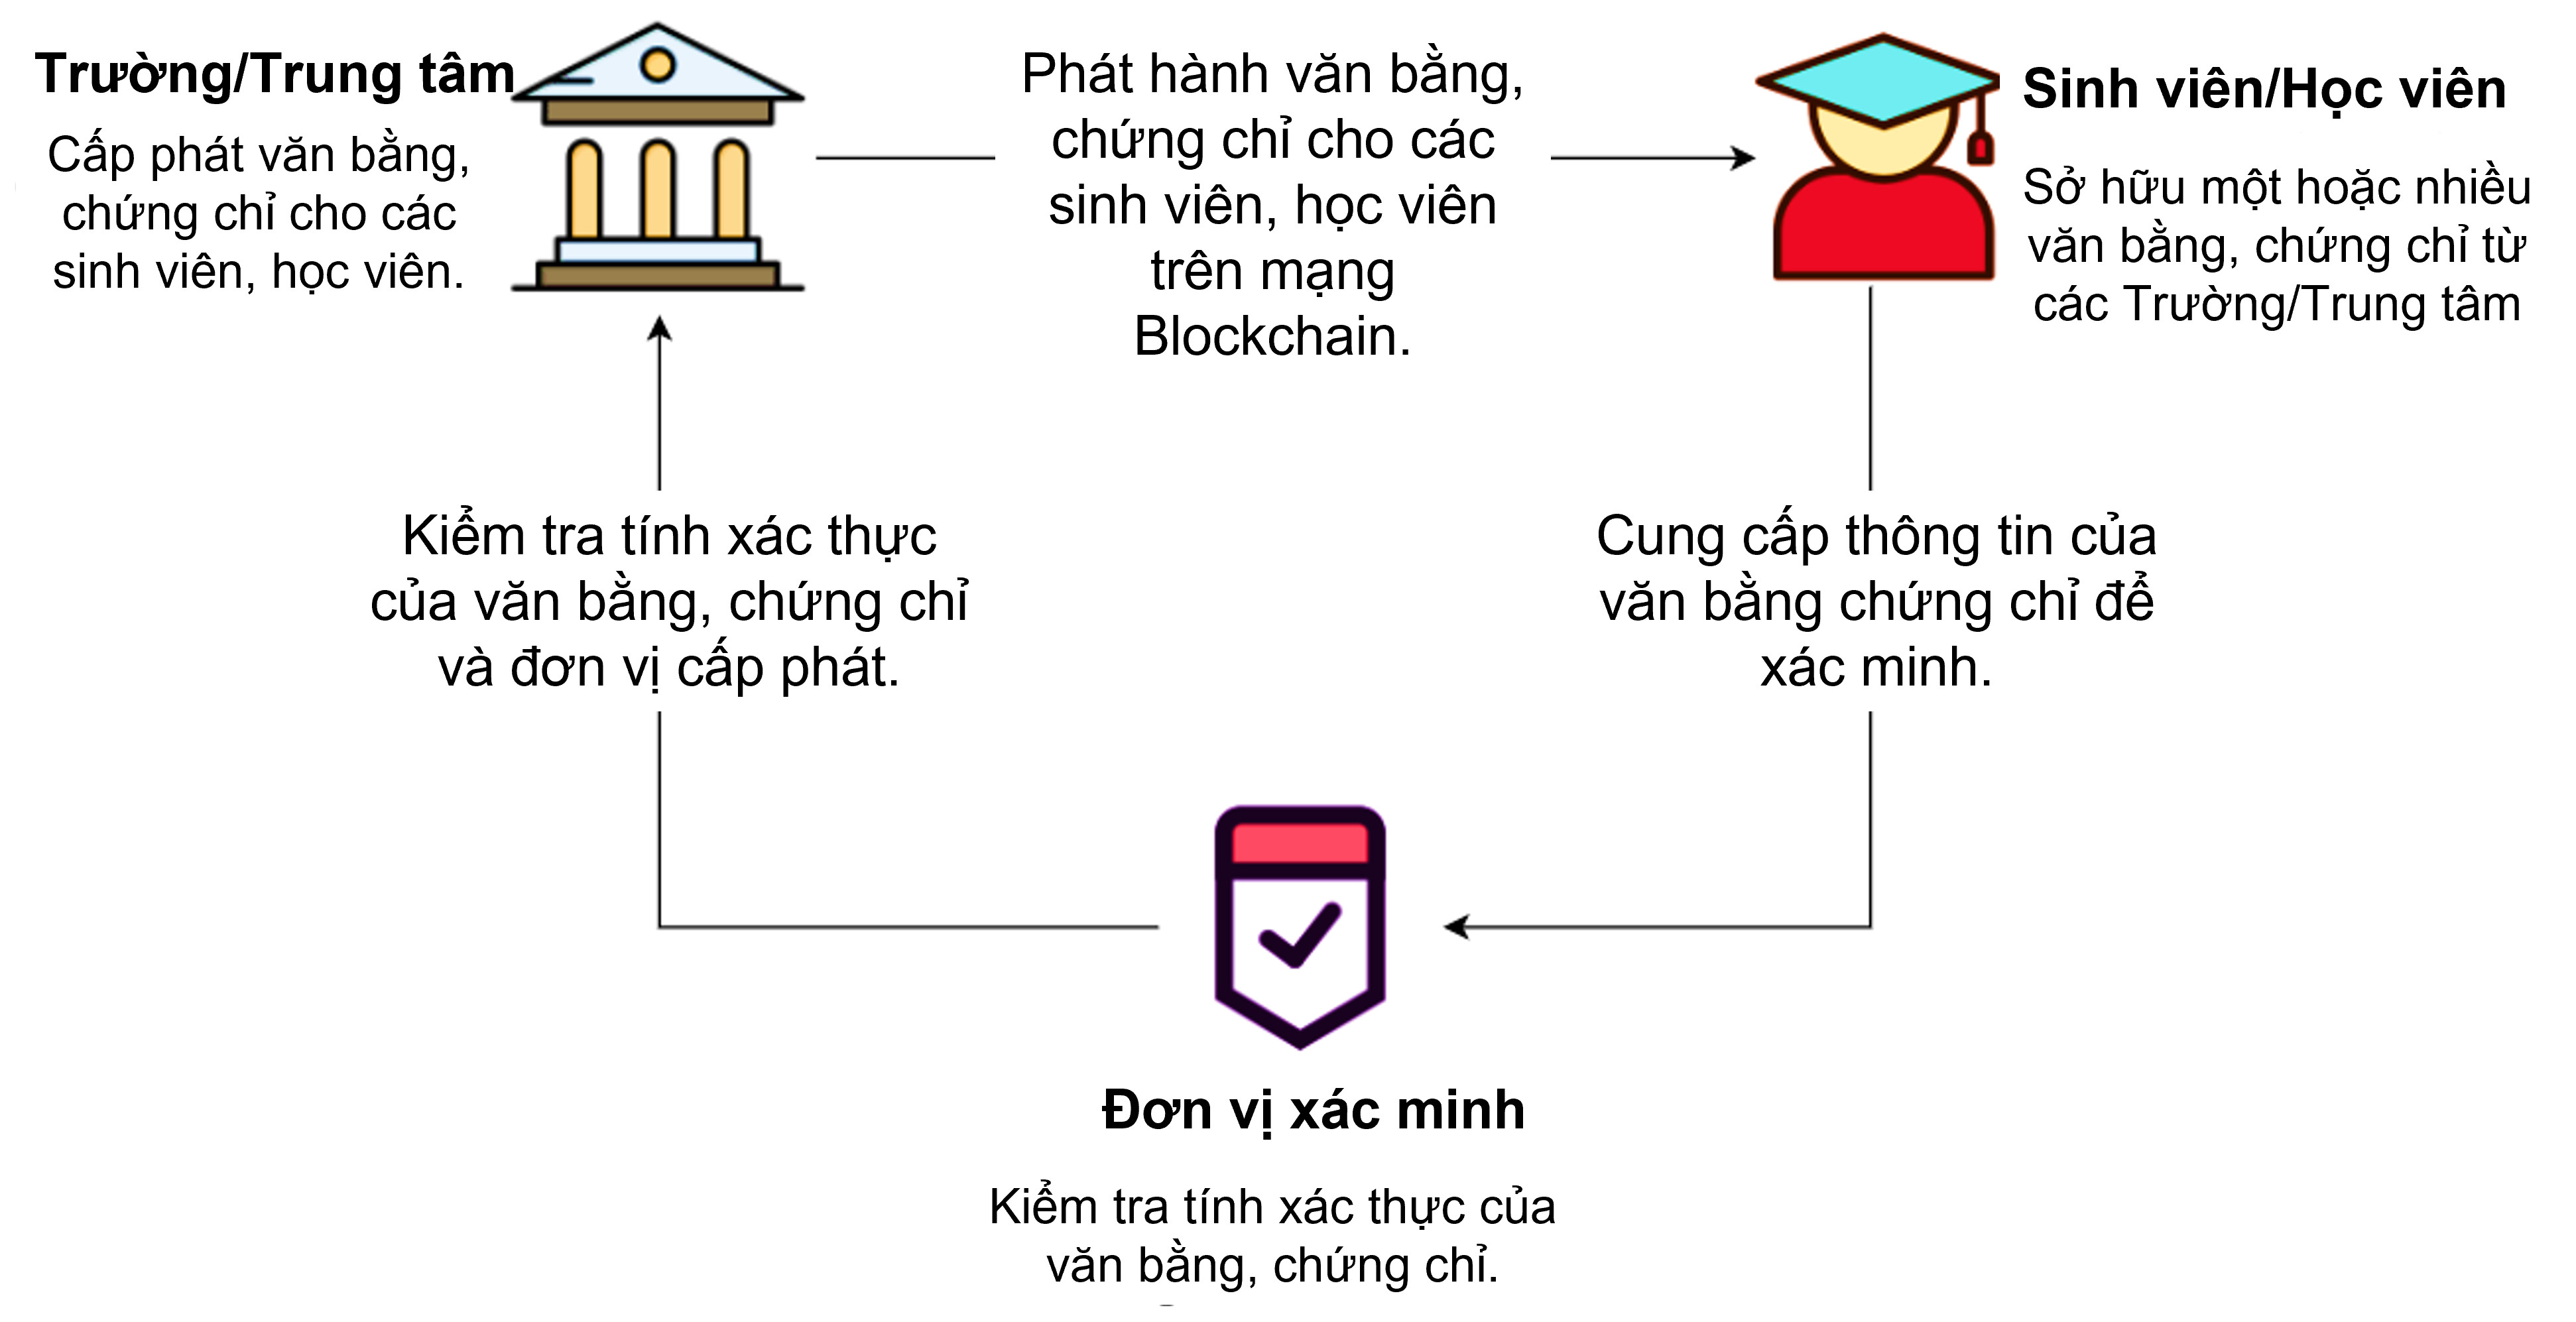
\includegraphics[width=.9\linewidth]{img/vbcc.jpg}
\caption{Sơ đồ bài toán quản lý VBCC}
\label{fig:vbcc}
\end{figure}

\section{Tổng quan giải pháp}

Nghiên cứu đề xuất một mô hình thử nghiệm ứng dụng Blockchain để đảm bảo tính an toàn thông tin VBCC và tính bí mật thông tin của người được cấp VBCC.
Hệ thống thực hiện việc ký số khi cấp VBCC và truy vấn dữ liệu Blockchain để xác thực VBCC. 
Kiến trúc hệ thống được mô tả như hình \ref{fig:vbcc_phanmem}.

\begin{figure}[htbp]
\centering
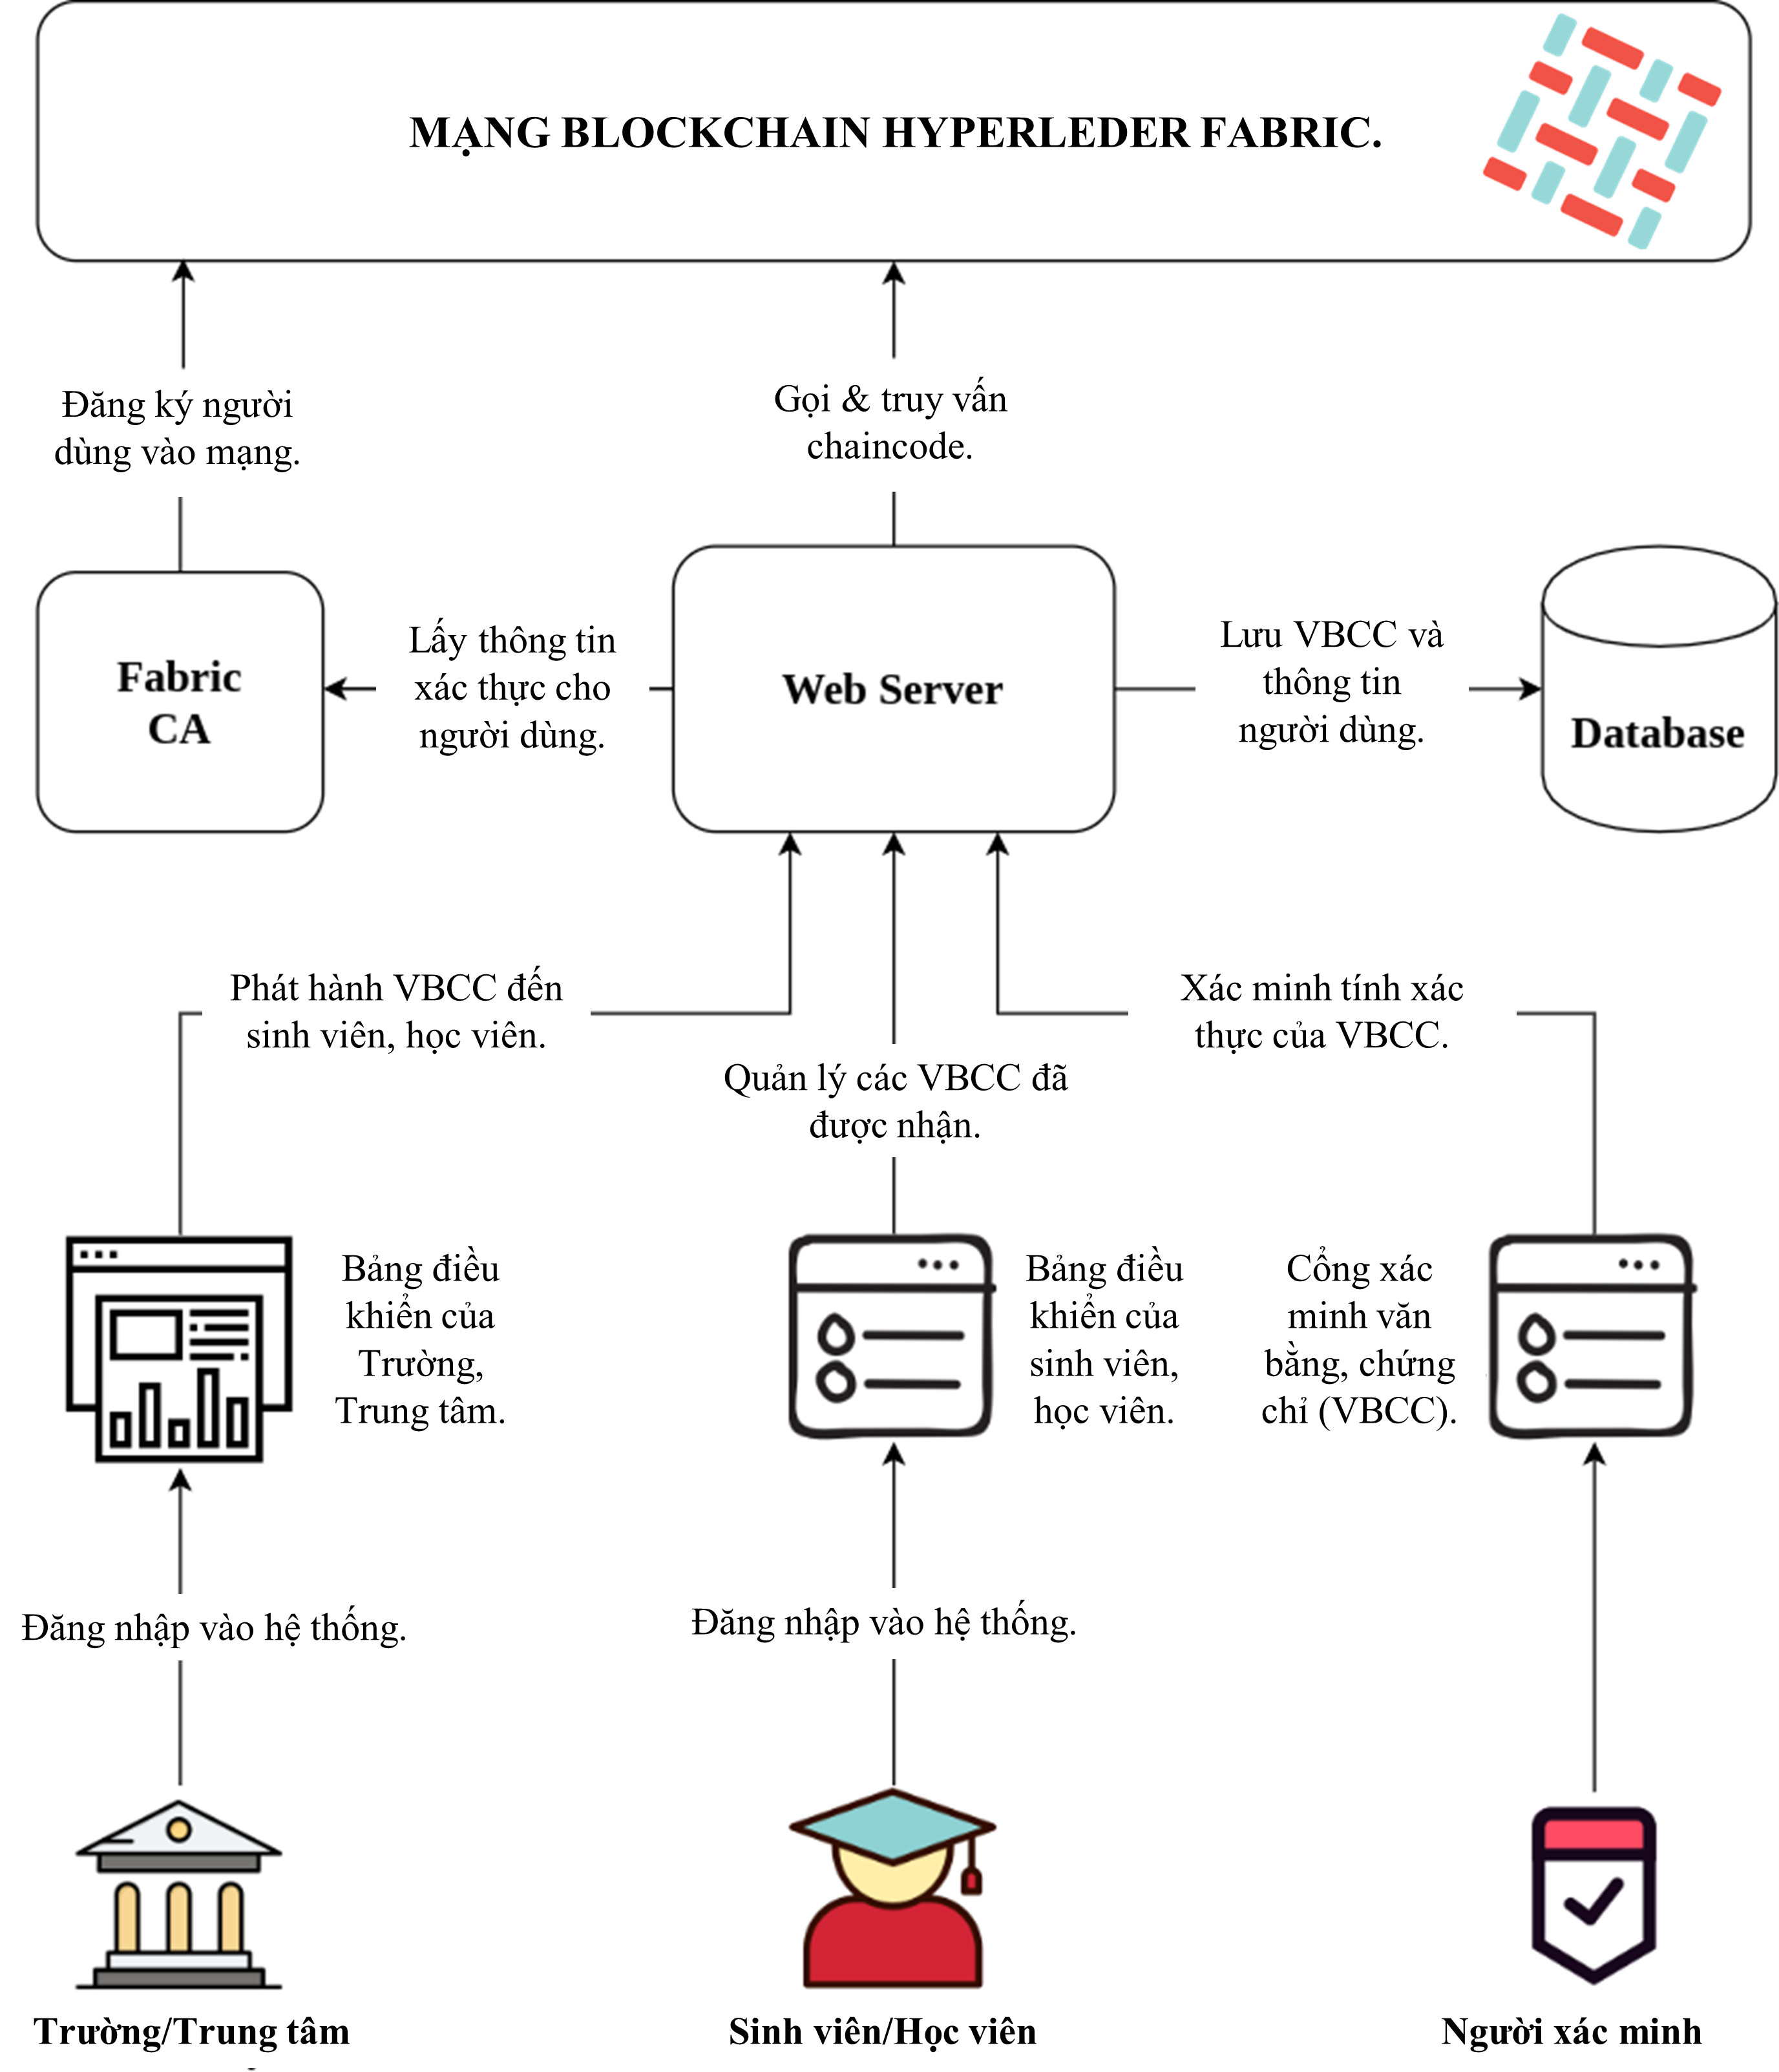
\includegraphics[width=.9\linewidth]{img/vbcc_phanmem.jpg}
\caption{Sơ đồ kiến trúc hệ thống}
\label{fig:vbcc_phanmem}
\end{figure}

Quy trình hoạt động của hệ thống được minh họa như hình \ref{fig:vbcc_diagram}.

\begin{figure}[htbp]
\centering
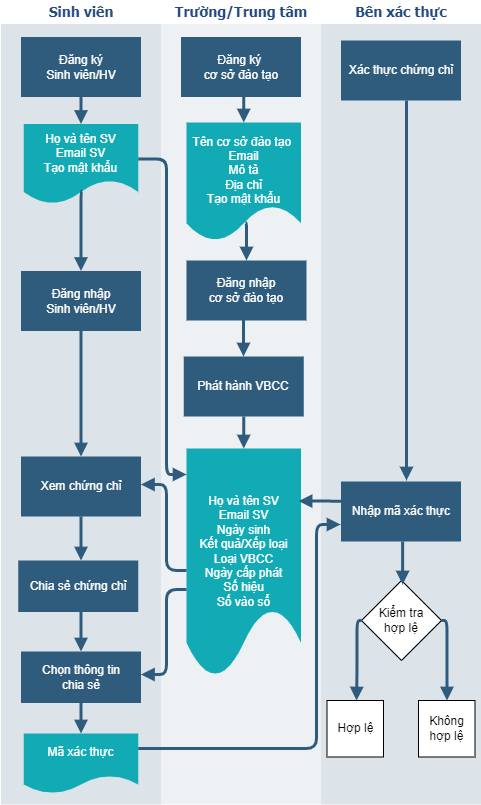
\includegraphics[width=.9\linewidth]{img/vbcc_diagram2.png}
\caption{Quy trình hoạt động của hệ thống}
\label{fig:vbcc_diagram}
\end{figure}

\subsection{Danh sách actor}

\begin{table}[H]
\caption{Danh sách actor}
	\label{table:actor}
	\begin{tabularx} {\textwidth} {|p{1cm}|p{3cm}|X|}
\hline
	ID & Tên actor & Mô tả \\ \hline
	A1 & Sinh viên &  là sinh viên/học viên nhận VBCC \\ \hline
	A2 & Trường học  & Trường/Đơn vị có quyền cấp VBCC \\ \hline
	A3 & Người xác minh  & Người/Đơn vị có nhu cầu xác minh VBCC \\ \hline
\end{tabularx}
\end{table}

\subsection{Danh sách Use Case}

\begin{table}[H]
\caption{Danh sách Use Case}
	\label{table:usecase}
	\begin{tabularx} {\textwidth} {|p{1cm}|p{1cm}|p{3cm}|X|X|}
\hline
		STT &	ID & Tên Use Case & Mô tả & Yêu cầu nghiệp vụ \\ \hline
		1 & U1	& Đăng nhập &Đăng nhập vào hệ thống để xác thực người dùng &Được mở rộng bởi tất cả \\ \hline
		2 & U2 & Đăng ký  & Đăng ký tài khoản vào hệ thống & Được mở rộng bởi tất cả\\ \hline
		3 & U3	&Cấp VBCC & Cấp VBCC có xác nhận chứng thực và ký số VBCC & \\ \hline
		4& U4	& Xem VBCC đã cấp& & Xem các VBCC  do Trường cấp \\ \hline
		5 & U5	&Xem VBCC đã nhận & Xem VBCC sinh viên đã nhận& \\ \hline
	6	& U6	&Chia sẻ thông tin VBCC &Chia sẻ thông tin VBCC & \\ \hline
		7& U7	& Xác thực VBCC &Xác minh tính xác thực của VBCC với nền tảng blockchain & \\ \hline
\end{tabularx}
\end{table}
\subsection{Thiết kế CSDL}

\subsection{Thiết blockchain}

\emph{Thông tin tài sản}

\emph{Các đối tượng}

\emph{Hợp đổng thông minh}

